\documentclass[../characterization.tex]{subfiles}
\graphicspath{{\subfix{../../../../images/}}}
\begin{document}
    \textbf{Scanning Electron Microscopy (SEM)}\cite{b12} is a powerful imaging technique used to examine the surface 
    morphology and composition of materials, including nanophosphors. It provides high-resolution images and 
    allows for detailed analysis of the sample's topography, particle size, shape, and surface features. SEM is 
    widely used in materials science, nanotechnology, biology, geology, and various other fields to investigate 
    the surface morphology and composition of nanophosphors and other materials. It offers high-resolution 
    imaging capabilities and provides valuable insights into the structural and surface properties of 
    nanophosphors, aiding in their characterization and understanding for various applications.
    \begin{Figure}
        \centering
        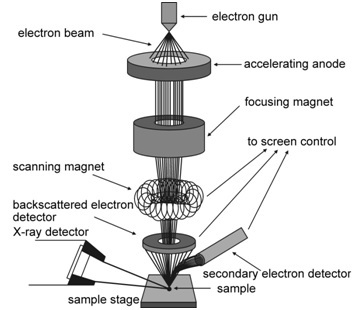
\includegraphics[width=0.6\linewidth]{sem.jpg}
        \captionof{figure}{Schematic diagram of Scanning Electron Microscope\cite{u12}}\label{fig:sem}
    \end{Figure}
    SEM uses a focused beam of high-energy electrons instead of light to interact with the sample. 
    The electron beam is generated from an electron source, typically a tungsten filament or field emission 
    source.The nanophosphor sample is typically mounted on a conductive substrate or coated with a thin 
    conductive layer, such as gold or carbon. This ensures that the sample can conduct electrons and avoids the 
    accumulation of charge during imaging.The electron beam is scanned across the surface of the sample in a 
    raster pattern. As the beam interacts with the sample, various signals are generated, including secondary 
    electrons (SE), backscattered electrons (BSE), and characteristic X-rays.It primarily utilizes secondary 
    electrons, which are low-energy electrons emitted from the surface of the sample due to the interaction with 
    the primary electron beam. These electrons provide information about the sample's surface morphology and 
    topography. Backscattered Electrons (BSE) are high-energy electrons that undergo elastic scattering after 
    interacting with the atomic nuclei of the sample. BSE imaging provides information about the sample's 
    composition, density variations, and atomic number contrast. The signals generated by the interaction of the 
    electron beam with the sample are detected by specialized detectors. These detectors collect the signals 
    and convert them into electrical signals, which are then processed to form images of the sample's surface. SEM 
    images can be further analyzed using dedicated software to measure particle size, distribution, and perform 
    quantitative analysis. Image processing techniques can enhance contrast, remove noise, and provide valuable 
    information about the sample's features.
\end{document}